\chapter{Methodology and experiment}

\cite{Gadiraju2015} categorize typically crowdsourced tasks into six top-level classes. Interesting classes within geospatial data is \textit{Verification and validation}, \textit{Interpretation and analysis} and \textit{Content creation}. There are examples of all three task classes in geospatial crowdsourcing. During imports of large datasets into OpenStreetMap, crowdsourcing is used to validate the new data. In humanitarian OpenSteetMap, they map areas during a crisis to support the help organizations through crowdsourcing, creating valuable content to the workers in the field. In a machine learning process, they are starting to use micro-tasks to both validate the created data and also create test data sets to the algorithms. \textit{Interpretation and analysis} tasks rely on the individual to use their interpretation skills during task completion. This is the task class used in this thesis during the survey. Is it safe to assume that individuals, both experienced and inexperienced, can interpret and analyse geospatial data presented to the on both map and in tables correctly? This is the main goal of the survey. 

\section{Survey}
This thesis will try to determine questions regarding micro-tasks containing geospatial data. Little research is done on how well inexperienced individuals solve micro-tasks when they involve map interaction and geospatial data. To the authors best knowledge, little, if any, research has been done on micro-tasks involving map interaction and geospatial interpretation and analysis. 

\section{Experiment}\label{sec:survey}
The survey is a part of this thesis. The survey is used to answer different hypothesis around geospatial micro-tasks. To be able to answer the hypothesizes three tasks containing the same two questions was developed. The questions will represent two different micro-tasks involving geospatial data, while the three tasks will vary the number of elements the participant will use to answer the questions with. The participant will always answer the two question's on six elements, but the tasks vary how many element's need to be handled at the same time. The variation of a number of elements in the tasks is to hopefully find out if or how much the number of elements in a micro-task effect how well people solves the task. 

When selecting the number of elements in the three different tasks the author decided to base this on cognitive load theory. Cognitive load theory refers to the total amount of mental effort being used in the working memory. Working memory is determined by the number of information elements that need to be processed simultaneously within a certain amount of time \citep{Barrouillet2007}. A heavy cognitive load can have negative effects on task completion, also the cognitive load that is imposed by a learning task is much higher for novices that for more advanced students \citep{Leppink2014a}.  

It is stated that the working memory has a limited capacity of seven plus or minus two elements (or chunks) of information when merely holding information and even fewer (ca four) when processing information \citep{Leppink2014a}. By choosing three elements in one task and six elements in the other task this paper can determine if the theories about the limited capacity of the human brain also apply to maps and geospatial data. The last task will only contain one element as a minimum cognitive load task. This can help answer how many elements a human can process when doing micro-tasks containing geospatial data. The goal is to determine a preferred number of elements within a micro-task to use when developing micro-tasks so that they are most efficient and accurate.

The “magical” number of 4 has been demonstrated to limit much of human information processing \citep{Mandler2013}. It is said that polygon comparison demand medium cognitive load \citep{Kiefer2016}, which is what the participants do in the first question in this survey. \cite{Kiefer2016} argues that high cognitive load may lead to less effective map reading and spatial orientation, as well as decreased spatial learning. Since polygon comparison doesn't demand high cognitive load, the task should at least not be too demanding on the one element task and the three elements task. A worry is that the inexperienced participants will have a bigger struggle than the experienced participants. The extraneous cognitive load imposed high for the inexperienced when solving problems, because their lack of prior knowledge of how to solve that type of problem forces them to resort to weak problem-solving strategies \citep{Leppink2014a}. By dividing the participants into experienced and inexperienced categories the results from the survey can help determine if geospatial micro-tasks are too demanding on inexperienced individuals. 

The survey will then contain three tasks, each task contains six elements but the tasks vary how many elements the participant need to handle at the same time. One task will serve the participant with one and one element, the task that demands the smallest cognitive load. The other task will serve the participant with three and three elements at the same time. This number is just under the limit of how much information humans can process. The last task will serve the participant with all the elements at the same time. This number exceeds the human capacity when processing information according to \cite{Leppink2014a}. 

There are two variable types used in this survey, dependent- and independent variables. The dependent variables are: time spent on each question and each task, the number of correctly chosen elements in both questions and also how difficult the participant though the task was. The independent variables are: number of elements in the task, experienced or inexperienced participant, gender, age and if the participant knows micro-tasking. 

\section[Building shapes]{Determining the building shapes}
Remote sensing is a tool or technique for extracting information about objects or geographic areas. All remote sensing images are subject to some form of geometric distortions. The distortions depend on how the data are obtained \citep{Toutin2004}.  In Norway, most remote sensing images are analysed manually. This is also the case in OpenStreetMap. When using remotely sensed images to create for instance building footprints, it's important to be aware of the distortions in these images. 

According to \cite{Fan2014}, there was over 77 million buildings in the OpenStreetMap (OSM) database in 2013. A study of the geometries of building footprints in the city Munich reveal a large diversity in the geometries \citep{Fan2014}, and this is probably not the only city with this kind of diversity. To evaluate the quality of the building footprints in OSM, the \cite{Fan2014} paper used four criterion's, completeness, semantic accuracy, position accuracy and shape accuracy. 

%These criteria will be used to create the building elements and conflicts used in the first question in the survey. The first question asks the participant to select the shape that fits the marked building on the map best. The goal is to create shapes that matches realistic cases that occur for instance in OSM. 

%Map matching is the process to identify correspondent features between two geospatial data sets, cannot be used to identify corresponding polygons in two building data sets \citep{Fan2014}.     

In the creation of the elements and conflicts used in the first question in the survey, the quality criterion's shape- and position accuracy were emphasized. The first question asks the participant to select the shape that fits the marked building on the map best. The goal is to create shapes that matches realistic cases that occur for instance in OSM. 

Shape accuracy evaluates how well the layer matches the building with reference to an aerial image. \cite{Fan2014} mentions three main reasons to why building footprints are simplified in OSM. First reason is because of the difficulties following building details when looking from a bird's-eye view. Second reason is the limited resolution on the Bing aerial image used during digitalization. The last reason that is mentioned is that the volunteers in OSM don't have the patience to digitalize a complicated footprint exactly as it is. Drawing two layers with one of them matching the building shape better than the other, the participant has to use an aerial image to determine which layer fits the building best. This will test if the participants manage to make correct shape judgements by only using an aerial image as reference. 

Position accuracy evaluates how well the coordinate value of a building relates to the reality on the ground. The correct layer will be drawn on the corresponding ground coordinates, while the conflicting layer will not match the ground. \cite{Fan2014} tested the accuracy of buildings in OSM, and concluded with an mean offset of 4.13 m. The low positional accuracy of OSM building footprints data is caused by the limited resolution of Bing map images. By combining shape- and position accuracy in some of the cases used in question one this study can also determine if participants manage to evaluate both factors. In this study the participants don't have available information about what the true ground coordinates are. Therefore position accuracy will be examined by shifting one of the layers. The correct positional accuracy will be at the building in the aerial image. 

\section{Web application}
This thesis used an online web-based survey to conduct the experiment. An online survey avoid the cost and effort of printing, distributing, and collecting paper forms. Many people prefer to answer a brief survey displayed on a screen instead of filling in and returning a printed form \citep{Ben2009}.   

In a self selected sample, which is some the case here, there is potentially a bias in the sample \citep{Ben2009}. %s168

\subsection{Technology}
React \\
Django \\
Postgis \\
AWS \\

\subsection{Architecture}

\begin{figure}[H]
	\centering
	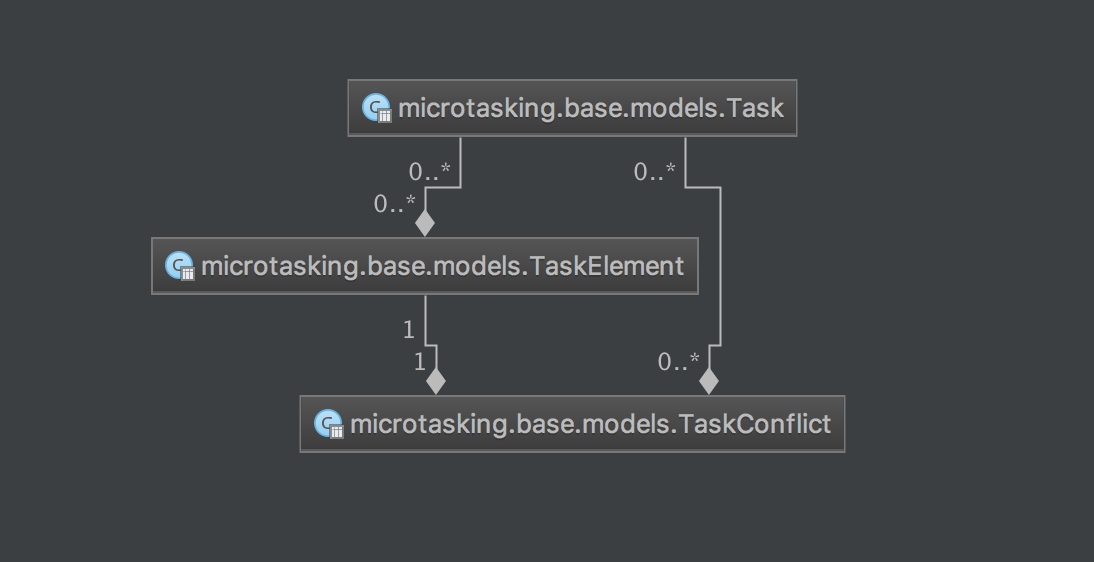
\includegraphics[width=0.7\linewidth]{fig/uml_diagram_task2}
	\caption[Task, UML diagram]{UML diagram, Task: Task Element and Task Conflict}
	\label{fig:umldiagramtask2}
\end{figure}


\begin{figure}[H]
	\centering
	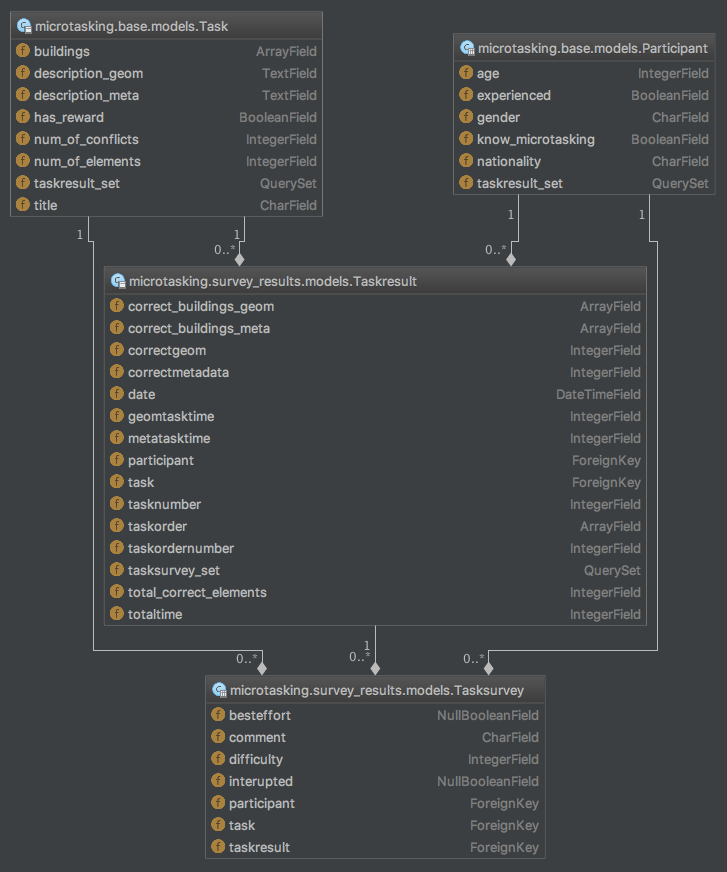
\includegraphics[width=0.8\linewidth]{fig/uml_diagram_taskresult}
	\caption[Survey result, UML diagram]{UML diagram, Survey result: Task result and Task survey}
	\label{fig:umldiagramtaskresult}
\end{figure}



\subsection{Graphical Interface}

\section{Pilot test}
It is important to pilot test the survey prior to actual use \citep{Ben2009}. A pilot test provides an opportunity to validate the wording of the tasks, do the participants understand the tasks? It also helps understand the time necessary for completing the survey, which should be communicated to the participants in prior to the survey \citep{Schade2015}. The pilot-test will be conducted with a small sample of users. Results from the pilot test are in this thesis used to do improvements to the actual survey, to the web application hosting the survey and to find errors or weaknesses in the database models.

After the pilot test, the usability was measured. The standard ISO 9241-11 suggests that measures of usability should cover effectiveness, efficiency and satisfaction \citep{ISO1998}. Measuring these three classes of metric can vary widely and makes it difficult to make comparisons of usability between different systems. "[...] just because a particular design feature has proved to be very useful in making one system usable does not necessarily mean that it will do so for another system" \citep{Brooke1996}. Usability in this thesis will be measured with the \textit{System Usability Scale}(SUS) because it gives a subjective measure of usability. The \textit{System Usability Scale} questionnaire consists of ten statements where the participants rate their agreement on a five-point scale \citep{Ben2009}. Subjective measure of usability is usually obtained through the use of questionnaire and attitude scales \citep{Brooke1996}. SUS was developed to be quick and simple, but also reliable enough to be able to compare performance changes between versions \citep{Brooke1996}. It is also easy to administer the participants through the usability test and it can be used on small sample sizes and still give reliable results \citep{Affairs2013}.  

The usability is important to measure. If the participants don't understand how the web application works, they will probably not do the survey since they then have to invest time in understanding what to do. %they will either exit the survey or answer the questions in the survey wrong. 
It is also important to get enough participants to do the whole survey and not quit halfway in frustration of not understanding it properly. The \textit{System Usability Scale} can effectively differentiate between usable and unusable systems \citep{Affairs2013}. 

\subsection{Execution of the pilot test}
The pilot test was conducted with a total of eight participants, five experienced and three non-experienced participants aged from 22 to 64 years. It started with a brief information about this study and the survey. They were told to talk out load during the survey, no help or guidance was given to the participants. The author observed the participants while they conducted the survey. The author took notes and watched if the participants understood the questions in the survey correctly. After the survey a \textit{System Usability Scale} questionnaire was answered by the participants. At the end, the participants were asked to give general feedback on the web application. The SUS score and the feedback were then used to determine the usability of the web application and to determine which improvements to be done.  

\subsection{Results from the pilot test}

- Did someone knew micro-tasking? Can we see something here?

The average SUS score was 84.64 out of 100. Anything above 68 is considered above average \citep{Affairs2013}. When adding the SUS score to an adjective rating will an score of 85.5 or higher be described as excellent \citep{Bangor2009}. A score of 84.64 is then described as good/excellent. This result gives a good indication that the web-application is user friendly. 

All participants thought that the instruction movie was confusing. It was short, the instructions went too fast and it lacked voice descriptions. The movie needed major improvements, an important discovery. The purpose of the movie is to give the participant an introduction to how to answer the two questions. It gives important instructions, especially for participants that are not used to working with maps on a web page. 

Overall feedback on question one was that it was difficult to understand which building was which and also when a building layer was selected or not. The lack of labels on the buildings was done on purpose to get the task as much as possible realistic. The process of selecting the best building layer needed improvements, it had to be clearer that selection was done by clicking on the layer on the map, not by using the layer control as some thought. This problem was added to the movie with voice description, describing in detail how a layer was selected. The design on the question one page was also improved by adding color to the text telling the participant which layer they had selected. 

Another feedback from one of the participants was that both question views had too much information and long sentences. The participant advised to shorten the sentences and to move some of the information to the movie. This request was fulfilled in the new movie. The task progress bar was also removed, during the eight pilot tests the author didn't notice that any of the participants looked at the task progress bar. The progress bar was thought of as an extra help to inform how many elements was left in the task. Only the survey progress bar on the top right was found necessary. 

The pilot test data was used to test some of the hypothesis to find errors or weaknesses in the databasemodel. The data was extracted with the help of Django QuerySets and saved in csv files. Some preliminary results can be seen in section \ref{sec:preliminalyresult}. There were a few errors and weaknesses found during the statistical tests. Changes to the database models was necessary, and the changes done are listed under: 

\begin{enumerate}
	\item Add foreign key from TaskResult model to TaskSurvey
	\item Added four other fields in TaskResult model
	\begin{itemize}
		\item Total correct elements 
		\item Task order
		\item Task number
		\item List of correctly chosen building numbers in both questions
	\end{itemize}
	\item Difficulty field in Tasksurvey model was changed from Char field to Integer field
\end{enumerate}

The additional fields will mainly help with creating plots to better interpret the data and to more easily visualize the different results. 

\subsection{Preliminary results}\label{sec:preliminalyresult}
The pilot-test data was not normally distributed, and doing statistical analysis on data from eight participants didn't seem relevant. The data was mapped in char plots, visualizing some trends. 

The two oldest participants spent almost twice as much time on the test than the younger. Maybe it was too much cognitive load on them. Learning a new application and at the same time understanding how to do the survey and answer the questions given to them. One of them were experienced and the other inexperienced, so this is a surprising result. Figure \ref{fig:allparticipantssortedageparticipantexclude4labelage} show the task results from all participants ordered by age. There are three entries per participant, so three and three bars are results from the same participant. Task 1 represents the task with one elements, task 2 the task with three elements and task 3 the task with six elements.

\begin{figure}[H]
	\centering
	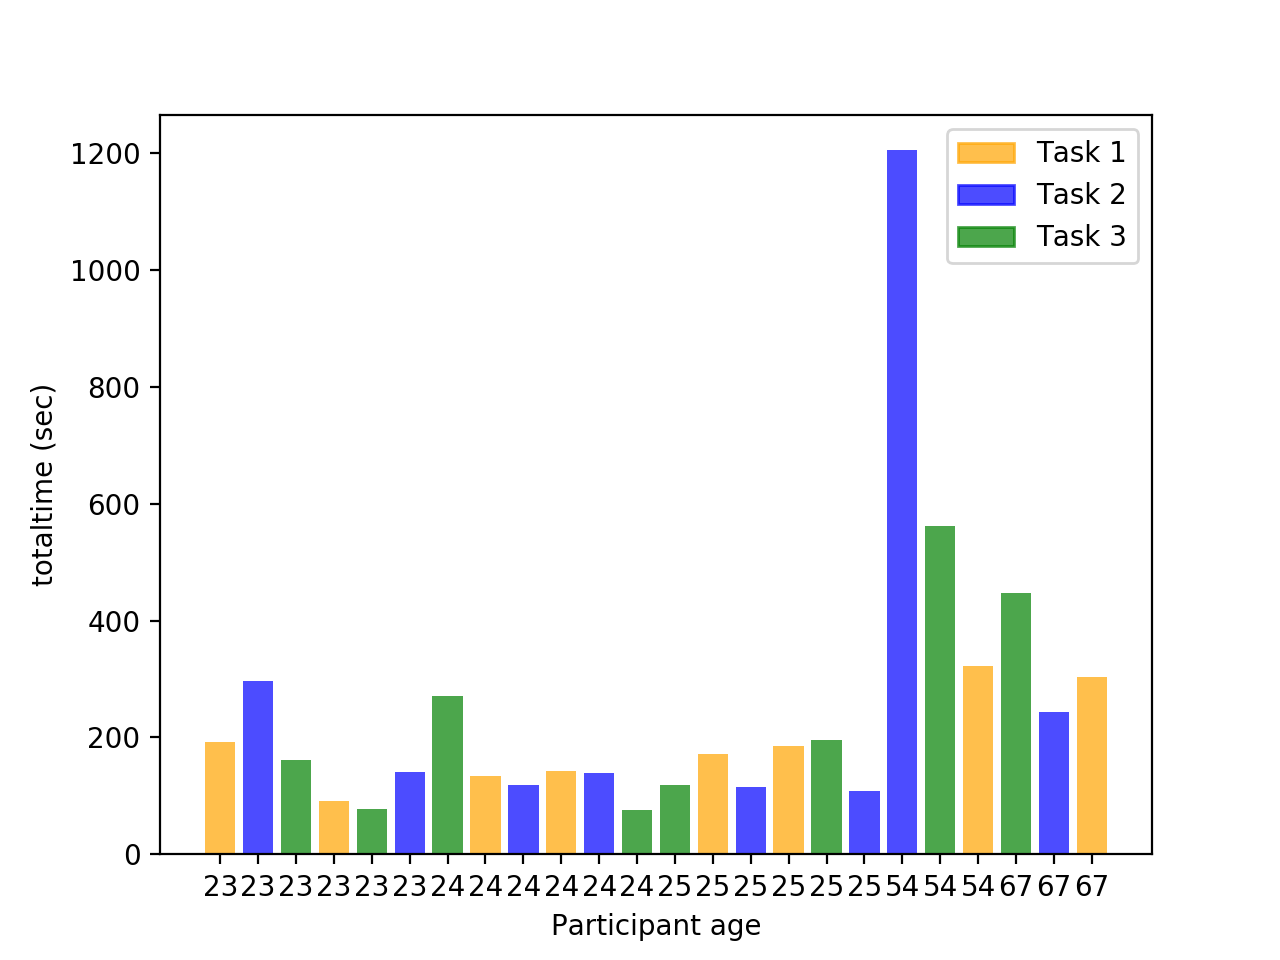
\includegraphics[width=0.7\linewidth]{fig/allParticipants_sorted_Age_Participant_exclude4_labelage}
	\caption[Total time, all]{Total time - all participants ordered by age}
	\label{fig:allparticipantssortedageparticipantexclude4labelage}
\end{figure}

Splitting the data into two groups, experienced and inexperienced, and then mapping totaltime and order by age plots can be seen in figures \ref{fig:experiencedexclude4labelagetotaltime} and \ref{fig:nonexperiencedexclude4labelagetotaltime}. Experienced participant had a mean time of 3 minutes and 24 seconds (204 sec) and inexperienced participants had a mean time of 5 minutes and 4 seconds (304 sec), almost 2 minutes difference. It is clear to see that the 54 year old participant's total time on task 2 is dramatically higher than the rest. By looking at figure \ref{fig:nonexperiencedexclude4labelagetotaltime}, two of the inexperienced participants spent less than 200 seconds on all their tasks.  

\begin{figure}[H]
	\centering
	\begin{subfigure}[b]{0.45\textwidth}
		\centering
		\includegraphics[width=\textwidth]{../../thesis-statisticmethods/statistic_analysis/figures/pilot-test/bar_chart/experienced_exclude4_labelage_totaltime}
		\caption{Experienced: Mean 204 sec}
		%, Std. 94 sec
		\label{fig:experiencedexclude4labelagetotaltime}
	\end{subfigure}
	\begin{subfigure}[b]{0.45\textwidth}
		\centering
		\includegraphics[width=\textwidth]{../../thesis-statisticmethods/statistic_analysis/figures/pilot-test/bar_chart/nonexperienced_exclude4_labelage_totaltime}
		\caption{Inexperienced: Mean 304 sec}
		%Std. 371 sec
		\label{fig:nonexperiencedexclude4labelagetotaltime}
	\end{subfigure}
	\caption[Total time, sorted]{Total time - ordered by age, splitted into experienced and inexperienced}
\end{figure}

The average time spent on the survey was 18 minutes. The two oldest participants used on average 33 minutes, while the rest of the participants spent on average 13 minutes to complete the survey. 

In the pilot-test the same building layers and meta data rows was used in all three tasks. At the end of the pilot-test the author asked the participants if they remembered the buildings and meta information in the last task. $\frac{7}{8}$ answered yes on the question. This information was important. If every participant does a better job at the last task the result will not be as useful. Even though the task order varies. Reading the data in figure \ref{fig:allparticipantssortedageparticipantexclude4labelage}, $\frac{6}{8}$ participants spent less time on the last task, even though the task order varied. This matches the number of participants who remembered the buildings and meta information from the previous tasks.

Total number of correctly chosen elements in each task is shown in figure \ref{fig:allparticipantssortedagetotalcorrect}. 

\begin{figure}[H]
	\centering
	\includegraphics[width=0.6\linewidth]{../../thesis-statisticmethods/statistic_analysis/figures/pilot-test/bar_chart/allParticipants_sorted_Age_totalcorrect}
	\caption[Total correct, ordered by age]{Total correct, both questions - ordered by age}
	\label{fig:allparticipantssortedagetotalcorrect}
\end{figure}

\begin{figure}[H]
	\centering
	\begin{subfigure}[b]{0.45\textwidth}
		\centering
		\includegraphics[width=\textwidth]{../../thesis-statisticmethods/statistic_analysis/figures/pilot-test/bar_chart/experienced_exclude4_labelage_geom}
		\caption{Experienced}
		\label{fig:experiencedexclude4labelagegeom}
	\end{subfigure}
	\begin{subfigure}[b]{0.45\textwidth}
		\centering
		\includegraphics[width=\textwidth]{../../thesis-statisticmethods/statistic_analysis/figures/pilot-test/bar_chart/nonexperienced_exclude4_labelage_geom}
		\caption{Inexperienced}
		\label{fig:nonexperiencedexclude4labelagegeom}
	\end{subfigure}	
\caption[Correcly chosen shapes, sorted]{Number of correctly chosen building shapes - splitted by experience}
\end{figure}

\section[Sample Size]{Determining the sample size}
The sample size is influenced by a number of factors, including the purpose of the study, population size, the risk of selecting a "bad" sample and the allowable sampling error \citep{Israel1992}. In this survey there are three possible ways of determining the sample size. 

\begin{figure}[h]
	\centering
	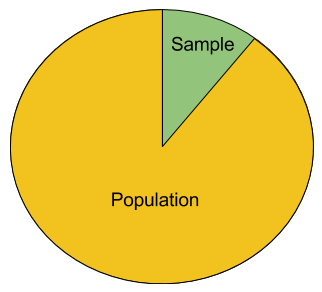
\includegraphics[width=0.35\linewidth]{fig/popsample}
	\caption{Population vs. sample}
	\label{fig:popsample}
\end{figure}

A sample is a collection of observations and is the subset of a population, illustrated in figure \ref{fig:popsample}. The population size in this survey is not easily determined. A population is the collection of individuals of a particular type \citep{Walpole2012}. All individuals with access to a computer and internet interested in contributing to micro-tasks is basicly the population. 

There are three possible ways of determining the sample size in this study. The first option is to use a sample size from a similar study. The risk is to repeat errors that were made in determining the sample for another study. The second option is to rely on published tables, depending on precision, confidence levels, and variability. According to \cite{Israel1992} table 1, a precision of 0.05, confidence level of 95\% and a size of population greater than 100'000, the necessary sample size is 400. If the precision is changed to 0.1, the sample size necessary increases to 100 \citep{Israel1992}. The numbers found in the table reflects the number of obtained responses. The last approach is to use formulas to calculate the sample size. The formulas requires the standard deviation and how much variance to expect in the response \citep{Smith2013}\citep{Israel1992}. \cite{Israel1992} mentions that the table gives a useful guide for determining the sample size, and that formulas are used if the study has a different combination of precision and confidence. This study will use the table result since the combinations matches this study.

It's important to mention that the quality of the sample is as important as it's size. The more variable the sampled data is, the larger the sample size is required \citep{Israel1992}. It's also desirable to choose a random sample, which means that the observations are made independently and random. The main purpose of using a random sample is to obtain correct information about the unknown population parameters \citep{Walpole2012}. 

%Results from the pilot-test can be used to determine the sample size. The sample size tells us how many responses that are needed to make inferences about a population as a whole \citep{Smith2013}. The formula for determining the sample size requires the standard deviation, how much variance to expect in the response \citep{Smith2013}. This standard deviation can be calculated from the pilot test results. Determining sample size is a very important issue because samples that are too large may waste time, resources and money, while samples that are too small may lead to inaccurate result. Equation \ref{eq:samplesize} show how to calculate the sample size, n. 

%\begin{equation}\label{eq:samplesize}
%n = [\frac{z_{\frac{\alpha}{2}}^2 \sigma (1-\sigma)}{e^2}]
%\end{equation}

%Using the results from all participants, excluding the training task, and using data from the column total time, the standardeviation is 184.8 and mean value 156.1 seconds.  
